\documentclass[12pt,a4paper]{extarticle}
\usepackage[T2A]{fontenc}
\usepackage[utf8]{inputenc}
\usepackage[russian]{babel}
\usepackage[margin=2.5cm]{geometry}
\usepackage{amsmath,amssymb,booktabs,float,graphicx}
\setlength{\parskip}{4mm}
\allowdisplaybreaks
\setlength{\emergencystretch}{1em}

\begin{document}
\author{Осипов Александр Б06-604}
\title{Лабораторная работа 1.2.5. Исследование вынужденной регулярной прецессии гироскопа}
\maketitle

\section{Цель}
Исследовать зависимость скорости прецессии от момента силы.

\section{Оборудование}
Гироскоп, секундомер, грузы, крутильный подвес, цилиндр, осциллограф, генератор.

\section{Ход работы}
\subsection{Прецессия}
\noindent $l=120$ мм, $g=9.81$ м/с$^2$.

\[\displaystyle \Omega = \frac{2 \pi N}{t}\]
\[\displaystyle \frac{\partial}{\partial N} \Omega{\left(N,t \right)} = \frac{2 \pi}{t}\]
\[\displaystyle \frac{\partial}{\partial t} \Omega{\left(N,t \right)} = - \frac{2 \pi N}{t^{2}}\]
\[\displaystyle \sigma_{\Omega} = \sqrt{\frac{4 \pi^{2} N^{2} \sigma_{t}^{2}}{t^{4}} + \frac{4 \pi^{2} \sigma_{N}^{2}}{t^{2}}}\]


\begin{center}
\begin{tabular}{rrrrr}
\toprule
m, г & N & t, с & M, Н м & $\Omega$, рад/с \\
\midrule
218.7 & 3.0 & 134 & 0.25745 & 0.14067 \\
218.7 & 2.0 & 90 & 0.25745 & 0.13963 \\
218.7 & 4.0 & 181 & 0.25745 & 0.13885 \\
218.7 & 4.0 & 179 & 0.25745 & 0.14041 \\
141.7 & 3.0 & 209 & 0.16681 & 0.09019 \\
141.7 & 3.0 & 209 & 0.16681 & 0.09019 \\
141.7 & 3.0 & 209 & 0.16681 & 0.09019 \\
340.3 & 3.0 & 87 & 0.4006 & 0.21666 \\
340.3 & 3.0 & 88 & 0.4006 & 0.2142 \\
340.3 & 3.0 & 87 & 0.4006 & 0.21666 \\
91.5 & 3.0 & 325 & 0.10771 & 0.058 \\
91.5 & 3.0 & 324 & 0.10771 & 0.05818 \\
116.1 & 2.5 & 214 & 0.13667 & 0.0734 \\
116.1 & 3.0 & 255 & 0.13667 & 0.07392 \\
\bottomrule
\end{tabular}

\end{center}

\subsubsection{Средние значения и их ошибка:}
\[
\sigma_{\overline{\Omega}}=\frac{s_\Omega}{\sqrt{k}}
\]
\begin{center}
\begin{tabular}{rrrrr}
\toprule
m, г & k & M, Н м & $\overline{\Omega}$, рад/с & $\sigma_\Omega$, рад/с \\
\midrule
91.5 & 2 & 0.10771 & 0.05809 & 9e-05 \\
116.1 & 2 & 0.13667 & 0.07366 & 0.00026 \\
141.7 & 3 & 0.16681 & 0.09019 & 0.0 \\
218.7 & 4 & 0.25745 & 0.13989 & 0.00041 \\
340.3 & 3 & 0.4006 & 0.21584 & 0.00082 \\
\bottomrule
\end{tabular}

\end{center}

\subsubsection{МНК:}

a - наклон прямой, L - момент импульса

\[\displaystyle \Omega = M a\]

\noindent $a=(0.54007\pm0.00095)\; (\text{Н м с})^{-1}$\par\vspace{3mm}


\begin{figure}[H]
\centering
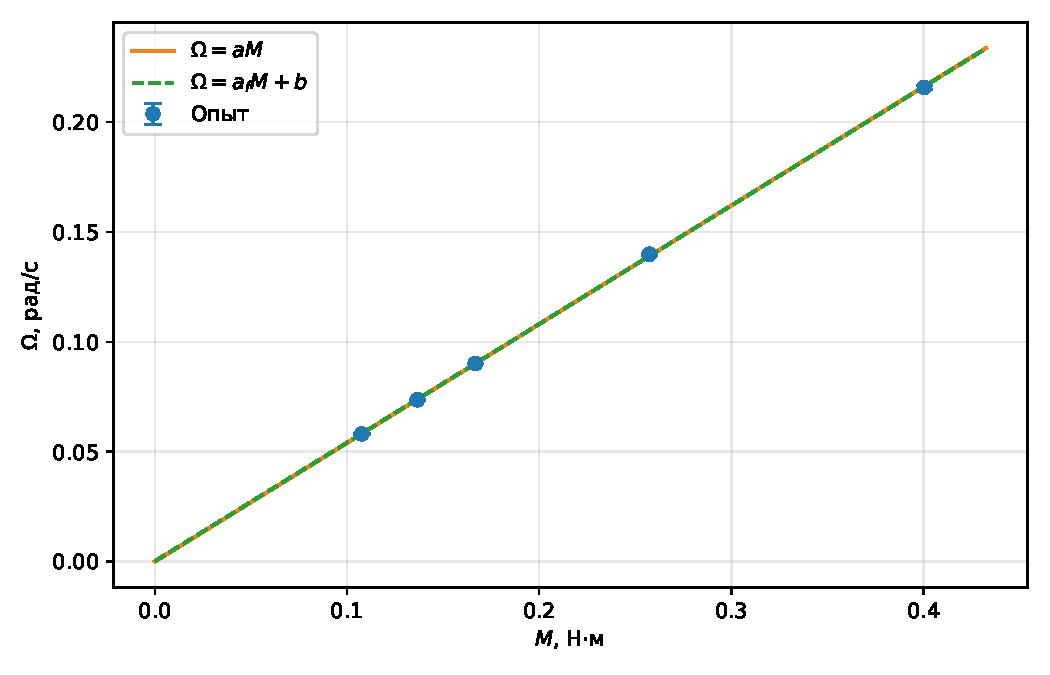
\includegraphics[width=0.85\linewidth]{generated/precession.pdf}
\end{figure}

\subsection{Момент инерции ротора}
\noindent $m_c=1.6158$ кг, $D_c=7.8$ см.

Ротор:
\begin{center}
\begin{tabular}{rrr}
\toprule
n & t, с & T, с \\
\midrule
10 & 31.76 & 3.176 \\
10 & 31.39 & 3.1390000000000002 \\
\bottomrule
\end{tabular}

\end{center}

Цилиндр:
\begin{center}
\begin{tabular}{rrr}
\toprule
n & t, с & T, с \\
\midrule
10 & 40.2 & 4.0200000000000005 \\
10 & 40.37 & 4.037 \\
\bottomrule
\end{tabular}

\end{center}

\[\displaystyle I_{0} = \frac{R_{c}^{2} T_{0}^{2} m_{c}}{2 T_{c}^{2}}\]
\[\displaystyle \frac{\partial}{\partial m_{c}} I_{0}{\left(m_{c},R_{c},T_{0},T_{c} \right)} = \frac{R_{c}^{2} T_{0}^{2}}{2 T_{c}^{2}}\]
\[\displaystyle \frac{\partial}{\partial R_{c}} I_{0}{\left(m_{c},R_{c},T_{0},T_{c} \right)} = \frac{R_{c} T_{0}^{2} m_{c}}{T_{c}^{2}}\]
\[\displaystyle \frac{\partial}{\partial T_{0}} I_{0}{\left(m_{c},R_{c},T_{0},T_{c} \right)} = \frac{R_{c}^{2} T_{0} m_{c}}{T_{c}^{2}}\]
\[\displaystyle \frac{\partial}{\partial T_{c}} I_{0}{\left(m_{c},R_{c},T_{0},T_{c} \right)} = - \frac{R_{c}^{2} T_{0}^{2} m_{c}}{T_{c}^{3}}\]
\[\displaystyle \sigma_{I_{0}} = \sqrt{\frac{R_{c}^{4} T_{0}^{4} \sigma_{m_{c}}^{2}}{4 T_{c}^{4}} + \frac{R_{c}^{4} T_{0}^{4} \sigma_{T_{c}}^{2} m_{c}^{2}}{T_{c}^{6}} + \frac{R_{c}^{4} T_{0}^{2} \sigma_{T_{0}}^{2} m_{c}^{2}}{T_{c}^{4}} + \frac{R_{c}^{2} T_{0}^{4} \sigma_{R_{c}}^{2} m_{c}^{2}}{T_{c}^{4}}}\]

\noindent $T_0=(3.1575\pm0.0185)\;\text{с}$\par\vspace{3mm}
\noindent $T_c=(4.0285\pm0.0085)\;\text{с}$\par\vspace{3mm}
\noindent $I_0=(7.549\pm0.094)\cdot10^{-4}\;\text{кг м}^2$\par\vspace{3mm}


\subsection{Частота вращения:}
\[\displaystyle \omega_{0} = 2 \pi \nu\]
\[\displaystyle \nu = \frac{1}{2 \pi I_{0} a}\]
\[\displaystyle \frac{\partial}{\partial a} \nu{\left(a,I_{0} \right)} = - \frac{1}{2 \pi I_{0} a^{2}}\]
\[\displaystyle \frac{\partial}{\partial I_{0}} \nu{\left(a,I_{0} \right)} = - \frac{1}{2 \pi I_{0}^{2} a}\]
\[\displaystyle \sigma_{\nu} = \sqrt{\frac{\sigma_{a}^{2}}{4 \pi^{2} I_{0}^{2} a^{4}} + \frac{\sigma_{I_{0}}^{2}}{4 \pi^{2} I_{0}^{4} a^{2}}}\]

\noindent $\nu=(390.4\pm4.9)\;\text{Гц}$\par\vspace{3mm}
\noindent $\nu_{\text{Лиссажу}}=400\;\text{Гц}$\par\vspace{3mm}
\noindent $\delta=-2.41\%$\par\vspace{3mm}
\noindent $\Omega_{\max}/\omega_0=8.62\cdot10^{-5}$\par\vspace{3mm}


\subsection{Момент трения}
\noindent $r=12.5$ см.
\[
\Delta\theta\approx\frac{h}{r},\qquad M_f\approx L\frac{\Delta\theta}{t}
\]
\[\displaystyle M_{f} = \frac{M h}{2 \pi N r}\]
\[\displaystyle \frac{d}{d h} M_{f}{\left(h \right)} = \frac{M}{2 \pi N r}\]
\[\displaystyle \sigma_{M_f} = \frac{M \sigma_{h}}{2 \pi N r}\]


\begin{center}
\[\displaystyle \sigma_{h} = \sqrt{\sigma_{1}^{2} + \sigma_{2}^{2}}\]
\[\displaystyle \sigma_{v} = \frac{\sigma_{h}}{t}\]
\[\displaystyle \sigma_{M_f} = \frac{M_{f} \sigma_{h}}{h}\]
\[\displaystyle \sigma_{\dot{\theta}} = \frac{\sigma_{h}}{r t}\]
{\raggedright здесь мы учитваем только систематическую погрешность цены деления линейки— 1 мм.\par}
{\raggedright Погрешность измерения рычага ротора не была указана \par}
\par\vspace{3mm}
\begin{tabular}{rrrrrr}
\toprule
m, г & N & h, см & $\sigma_h$, см & $M_f$, мН м & $\sigma_{M_f}$, мН м \\
\midrule
320.3 & 3.0 & 2.5 & 0.071 & 4.001 & 0.113 \\
320.3 & 3.0 & 2.0 & 0.071 & 3.201 & 0.113 \\
116.1 & 2.5 & 6.0 & 0.071 & 4.176 & 0.049 \\
116.1 & 3.0 & 4.5 & 0.071 & 2.61 & 0.041 \\
\bottomrule
\end{tabular}
\par\vspace{5mm}

\end{center}

\section{Вывод}

Измерена угловая скорость прецессии гироскопа, его момент инерции относительно оси. 
ВЫведена линейная зависимость угловой скорость от момент сила приложному 
перпендикулярно оси вращения гироскопа.

\end{document}
